\section{Diseño del sistema}\label{sec:diseno_del_sistema}

En la figura~\ref{fig:chapter_1.overview} vimos un esquema general del sistema, el cual recibe documentos en formato
PDF y genera objetos que contienen la información más importante de los mismos.
Dependiendo del tipo de documento, la información contenida en estos objetos puede variar.
En la figura~\ref{fig:chapter_1.specific_b} mostramos que se va a incluir también el desarrollo de dos interfaces, una
web y una de línea de comandos.
En esta sección profundizaremos en el diseño de la arquitectura de este sistema.
En la figura~\ref{fig:chapter_4.1.overview} vemos que el sistema tiene dos componentes principales: el componente
\textit{Generator} y el componente \textit{Reader}.

\begin{figure}[ht]
    \begin{center}
        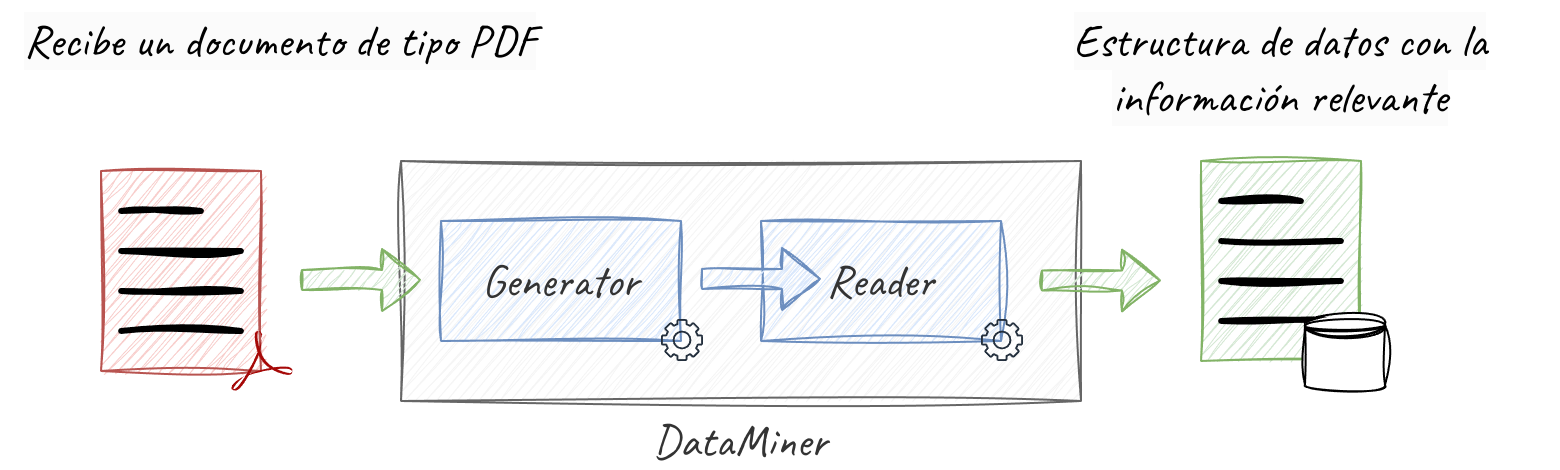
\includegraphics[width=\textwidth]{./chapter/4/images/chapter_4.1.overview}
        \caption{Esquema de los componentes principales}
        \label{fig:chapter_4.1.overview}
    \end{center}
\end{figure}

\subsection{Componente \textit{Generator}}\label{subsec:chapter_4.generator_component}

La responsabilidad de este primer componente, el \textit{Generator} es convertir archivos de cualquier formato en una
representación en texto plano con el contenido del mismo.
Tal y como se ve en la figura~\ref{fig:chapter_4.1.generator_component_uml} el componente consta de cuatro tipos
diferentes de elementos.

\begin{figure}[ht]
    \begin{center}
        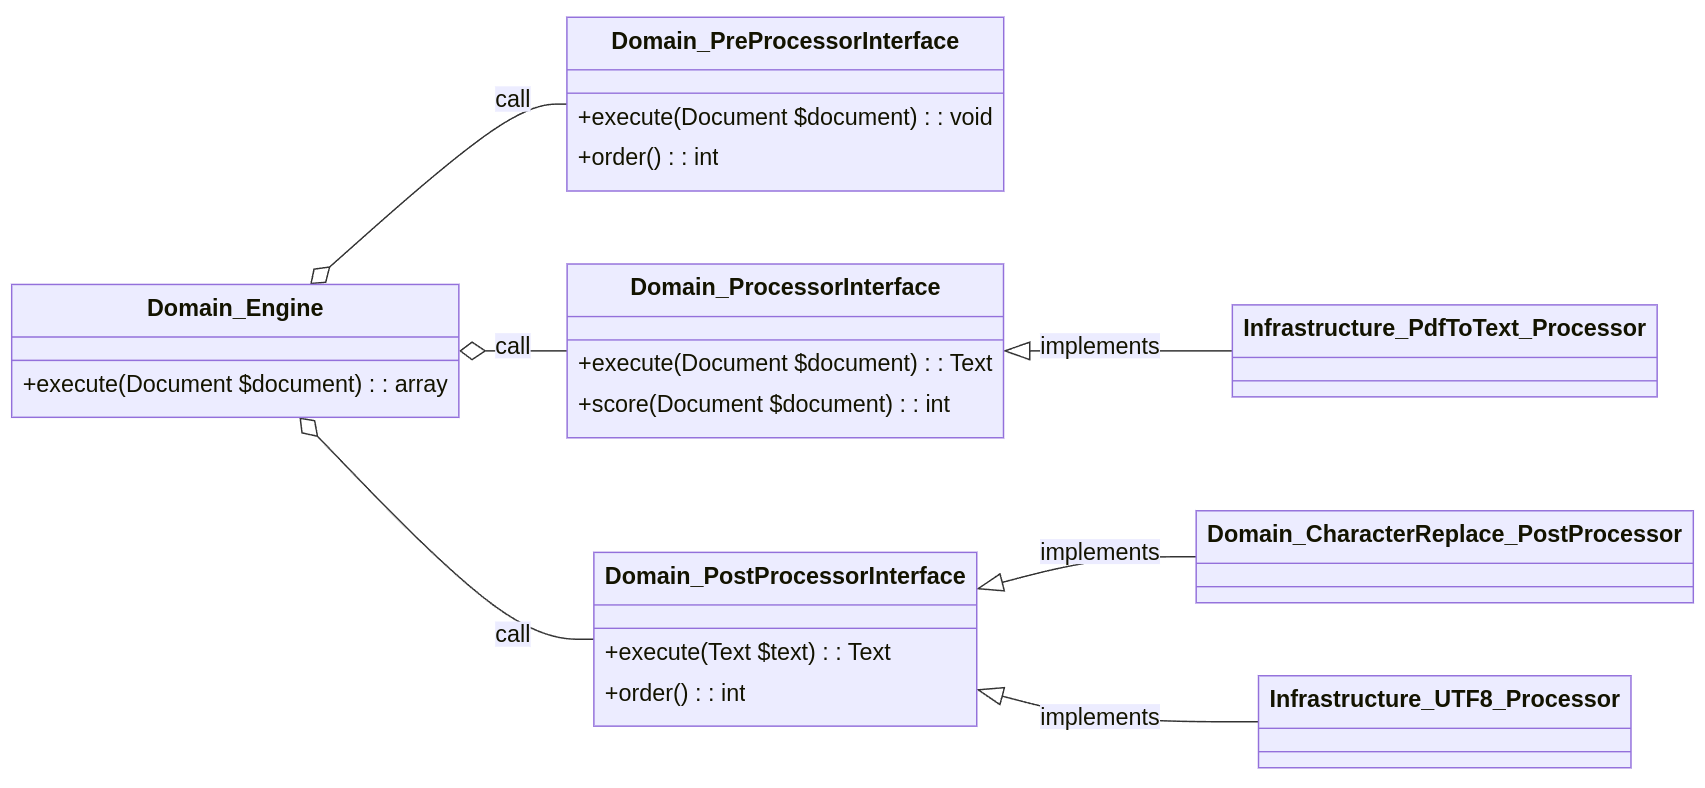
\includegraphics[width=\textwidth]{./chapter/4/images/chapter_4.1.generator_component_uml}
        \caption{Diagrama UML del componente \textit{Generator}}
        \label{fig:chapter_4.1.generator_component_uml}
    \end{center}
\end{figure}

Es importante destacar que salvo el \textit{Engine}, el resto de elementos son intercambiables, y dependiendo del caso
de uso, pueden utilizarse los componentes descritos en este TFG, o ser necesaria la implementación de otros nuevos.

El motor o \textit{Engine} es el corazón del componente.
Es el encargado de hacer las llamadas a los demás elementos registrados en el mismo coordinando cuáles y en que
orden deben ser llamados.

Los \textit{preprocesadores} preparan el documento original para facilitar su conversión a texto.
En esta implementación no se ha desarrollado ningún preprocesador, ya que no ha sido necesario para los casos de uso
previstos.

Los \textit{procesadores} realizan la conversión efectiva del documento a texto.
Funcionan mediante un sistema competitivo donde varios procesadores evalúan su propia aptitud para manejar el documento
en cuestión, seleccionando cuál es el más adecuado para llevar a cabo la tarea.

En la figura~\ref{fig:chapter_4.1.generator_component_processors} puede verse un ejemplo.
El \textit{Engine} pretende convertir un fichero PDF en texto y tiene registrados dos procesadores, el
\textit{MP3Processor} y el \textit{PDFProcessor}.

Primero realiza una llamada a \textit{MP3Processor}, el cual evalúa el documento y responde con una puntuación
de -1, lo cual significa que no es capaz de procesar este tipo de documento.

A continuación realiza una llamada a \textit{PDFProcessor}, el cual evalúa el documento y responde con una puntuación
de 90, lo cual significa que es adecuado para procesar este tipo de documento.

\begin{figure}[ht]
    \begin{center}
        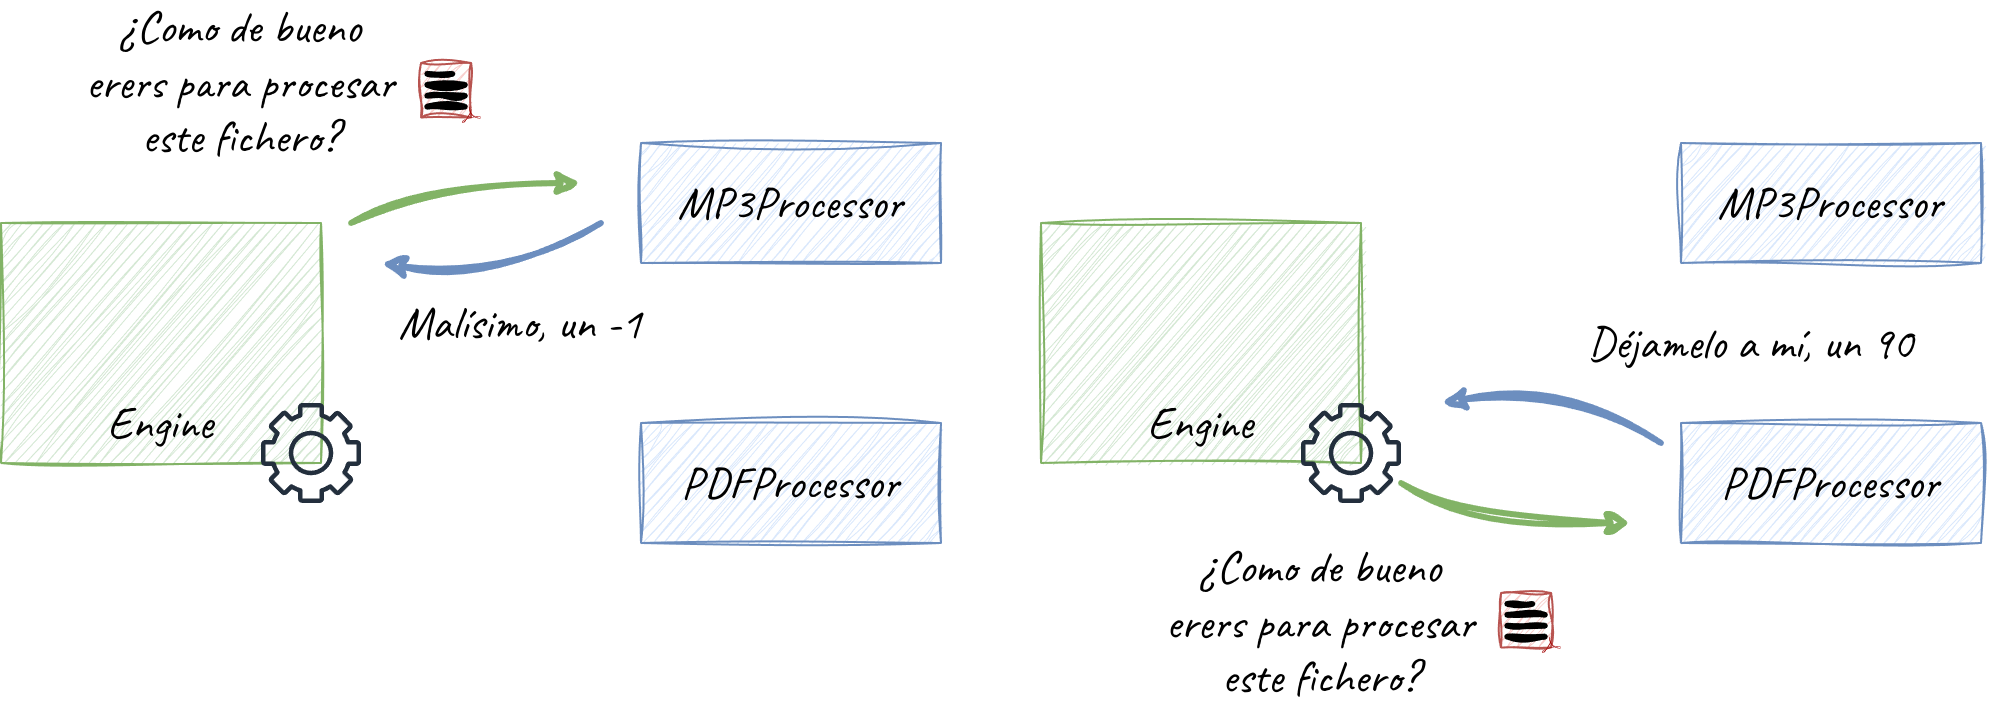
\includegraphics[width=\textwidth]{./chapter/4/images/chapter_4.1.generator_component_processors}
        \caption{Competición entre procesadores en el componente \textit{Generator}}
        \label{fig:chapter_4.1.generator_component_processors}
    \end{center}
\end{figure}

Si existieran más procesadores registrados, se irían invocando secuencialmente, para que evaluaran como de adecuados
son para procesar ese tipo de documento.
Finalmente, una vez que todos los procesadores han sido invocados, el \textit{Engine} enviará el documento al procesador
que haya respondido con una puntuación más alta.

Como puede verse, es fácil añadir soporte a nuevos tipos de documentos.
Se podría añadir soporte para documentos escaneados, simplemente añadiendo un procesador que utilizara una tecnología
de reconocimiento de caractéres u \textit{Optical character recognition} (OCR) como por ejemplo \textit{Tesseract}
~\cite{url_tesseract}.

El \textbf{Requisito 1} definido en el capítulo~\ref{ch:chapter_1} para este proyecto era ``convertir documentos PDF
en documentos de texto''.

El procesador \textit{PDF To Text Processor} es el responsable de esta tarea mediante llamadas a una tecnología que se
encuentra en la capa de infraestructura, en este caso
\textbf{Pdf to Text}~\cite{url_pdftotextl}.
Añadiremos más detalles sobre como fue la implementación de este procesador en la
sección~\ref{sec:implemetacion_y_programacion} Implemetación y programación.


Los \textbf{postprocesadores} perfeccionan el texto generado, realizando los ajustes necesarios, lo que mejora la
calidad del texto resultante.

Los postprocesadores se llaman secuencialmente.
El primer postprocesador recibe como entrada la salida del procesador ejecutado.
Los siguientes postprocesadores reciben como entrada la salida del postprocesador anterior.

En esta implementación, se han desarrollado los siguientes postprocesadores:

\begin{itemize}
    \item \textbf{UTF8 PostProcessor}: Algunos documentos pueden contener caracteres no UTF8. Como este tipo de
    caracteres pueden generar problemas, este procesador los reemplazará por caractéres equivalentes en UTF8.
    \item \textbf{Character Replace PostProcessor}: Después de eliminar los caracterés no UTF8 se detectó que algunos
    caracteres todavía podían resultar problemáticos, asi que se implementó un nuevo procesador capaz de reemplazar
    caracteres problemáticos, por otros equivalentes.
    En este caso se cambió el carácter \textit{\textbackslash f}, salto de página, por el carácter
    \textit{\textbackslash n} salto de línea.
    \item \textbf{Word Limit PostProcessor}: Más adelante en la implementación del componente \textit{Reader}, y debido
    al uso de las tecnologías implementadas en el mismo, se vio que documentos con textos demasiado largos podían
    generar errores.
    Es por esto que se decide implementar este procesador que trunca el texto después de las primeras N palábras.
\end{itemize}

\subsection{Componente \textit{Reader}}\label{subsec:chapter_4.reader_component}
El componente Reader es el responsable del proceso de interpretación y procesamiento del texto plano obtenido a
partir de la salida del componente \textit{Generator} descrito en la subsección anterior.

Tal y como se ve en la figura~\ref{fig:chapter_4.1.reader_component_uml} el componente consta de dos tipos diferentes de
elementos: El motor o \textit{Engine} es el corazón del componente.
Es el encargado de hacer las llamadas a los demás elementos registrados en la aplicación, en este caso únicamente los
procesadores.

\begin{figure}[ht]
    \begin{center}
        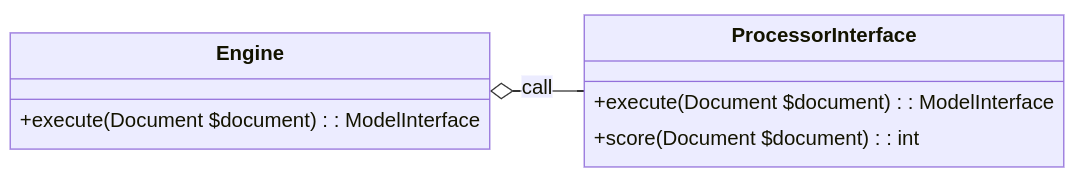
\includegraphics[width=\textwidth]{./chapter/4/images/chapter_4.1.reader_component_uml}
        \caption{Diagrama UML del componente \textit{Reader}}
        \label{fig:chapter_4.1.reader_component_uml}
    \end{center}
\end{figure}

\subsubsection{Motor}

Los \textbf{procesadores} organizados en una única capa,  operan bajo el mismo mecanismo competitivo descrito en la
subsección \ref{subsec:chapter_4.generator_component} Componente\textit{Generator}.

Cada uno de estos procesadores es invocado secuencialmente para evaluar su idoneidad en el manejo de un tipo de
documento específico.

Una vez seleccionado, el procesador elegido procede a ejecutar una serie de tareas que incluyen la identificación y
extracción de la información clave.

En esta implementación, se han desarrollado los siguientes procesadores:

\begin{itemize}
    \item \textbf{Residential Lease Processor}: Es adecuado para evaluar contratos de arrendamiento de vivienda entre
    particulares tal y como indicamos en \textbf{Requisito 2}.
    \item \textbf{Vehicle Sale And Purchase Processor}: Es adecuado para evaluar contratos de compra venta de vehículo
    entre particulares tal y como indicamos en \textbf{Requisito 3}.
\end{itemize}
